% ============================================================================
% ATML PA1 - Beyond IID
% EE-5102 / CS-6304, Fall 2026
% ============================================================================

\documentclass{article}

\usepackage[final,main]{neurips_2026}
\usepackage{enumitem}
\usepackage[utf8]{inputenc}
\usepackage[T1]{fontenc}
\usepackage{hyperref}
\usepackage{url}
\usepackage{booktabs}
\usepackage{amsfonts}
\usepackage{amsmath}
\usepackage{nicefrac}
\usepackage{microtype}
\usepackage{graphicx}
\usepackage{subcaption}
\usepackage{xcolor}

\graphicspath{{../figures/}{figures/}}

\title{Beyond IID: Inductive Biases, Domain Adaptation, Domain Generalization and Open-Set Recognition}

\author{%
  Talha \\
  \texttt{28100131} \\
  EE-5102 / CS-6304, Fall 2026 \\
}

\begin{document}

\maketitle

% ============================================================================
\begin{abstract}
In theory, for an input to be classified as accurately as possible, the
representation it receives via a learned model should encode information
sensitive to the nature of its true label, and not information that is
useless to its correct classification. We test this across four regimes:
independent intervention experiments on frozen backbones (STL-10),
unsupervised domain adaptation and domain generalization (PACS), and
open-set recognition (CIFAR-10/100). Going in order and covering the most
prevalent result from each regime, four independent interventions were
applied on STL-10: one focusing on colour bias, the other on shape bias and
the last two on patch shuffling and translation. The results showed
decreasing reliance on surface appearance from ResNet to ViT to CLIP as per
these numbers: colour gap ($-2.6$ / $-1.0$ / $-0.2$) and shape bias
(56.21 / 79.31 / 82.78). Translation and patch shuffling exposed the
structural biases of the architectures: ResNet-50 degraded least under
translation (an accuracy reduction of $-0.028$ per pixel) and ViT-B/16 least
under patch shuffling ($-7.0$ drop in accuracy). Using PACS with Sketch as
the target domain, DAN reduced domain separability to 83.52 but had the worst
target accuracy at 58.56, while DANN left it at 98.63 and had the best target
accuracy at 80.55. In a similar context but in an even lower data regime,
with no images of the target sketch domain used during training, the model
with the lowest domain separability, DAN-DG at 54.67 against a 33.3 floor,
had the worst target accuracy at 4.07, even below the 14.3 floor. In open-set
recognition (OSR) on CIFAR-10 with CIFAR-100 images being the unknowns,
PROSER reduced its placeholder loss to 0.0000 by epoch 30 but scored 85.58 on
all-unknown AUROC, below the 86.01 of the vanilla baseline it got fine-tuned
from. As such, the consensus was that each method that achieved its proxy
directive successfully performed worse on the goal that proxy was meant to
facilitate, suggesting that progress on an alignment or rejection proxy is
not evidence of progress on the goal.

\textbf{Repository:} \url{https://github.com/TalhaShoyo10/PA1_28100131}
\end{abstract}

% ============================================================================
\section{Introduction}
\label{sec:intro}

The standard regime for supervised model training assumes that both train and
test data are drawn IID from the same underlying distribution over a fixed
label space. This assumption fails under deployment conditions, which are
likely to test a model against inputs sampled from distributions (domains)
that differ from those the training inputs were drawn from. Additionally,
deployment can expose models to open-set situations, where the model must
classify inputs that fall outside the label set seen during training. This
experimental analysis studies methods that counter both of these restricting
assumptions.

To characterise what a representation actually depends on, Task 1 applies
controlled interventions to the inputs of three frozen backbones (ResNet-50,
ViT-B/16 and CLIP ViT-B/32), measuring how each degrades when colour,
texture, absolute position and global arrangement are individually disrupted.
Tasks 2 and 3 then test whether that dependence can be corrected: Task 2
compares a source-only baseline against DAN, DANN and CDAN when unlabelled
target data is available, while Task 3 compares ERM against DAN-DG and SAM
when no target data exists at all. Finally, Task 4 addresses the open-set
case, comparing a vanilla classifier against GCSC, which tests whether a
better closed-set classifier rejects better as a side effect, and PROSER,
which adds placeholder classes trained to represent the unknown.

Each of the four tasks carries four research questions. Though each is
addressed in its own subsection, they follow a sequence of recurring themes:
what a representation depends on, whether reducing a proxy metric improves
performance on the goal it stands in for, whether aggregate gains mask
per-class failures, and which variable can be identified as the causal factor
behind an observed difference in model performance.

% ============================================================================
\section{Experimental Setup}
\label{sec:setup}

Every experiment has a set of YAML files for configuration that are seeded
with 6304, so each split and permutation is deterministic. The resulting
splits are committed as manifests and each run records its resolved
configuration, git commit, library versions and device, so any reported
number traces back to the code iteration that produced it. Each experiment
was run once (no margin of error was determined), so differences of one or
two points in model performance on the same task should not be interpreted as
significant.

Task 1 evaluates three frozen backbones, ResNet-50, ViT-B/16 and CLIP
ViT-B/32, on a 500-image class-balanced subset of the STL-10 test split, with
linear heads trained on a stratified 80/20 split of the official train
partition. Tasks 2 and 3 share an experimental setup configured by a PACS
protocol module covering splits, transforms, batch composition and optimizer
settings: both fine-tune an ImageNet-pretrained ResNet-18 end-to-end with
domain-balanced batches of eight images per source domain, and both select
checkpoints based on the mean macro-F1 score on the validation subset of the
source domains alone. Additionally, the ERM baseline of Task 3 is the
source-only checkpoint of Task 2, so that both tasks have identical baseline
weights. The two differ only in what is available during training: Task 2 may
use unlabelled Sketch images, Task 3 may not. Task 4 uses the CIFAR variant
of ResNet-18. The standard network's first layer applies a 7$\times$7
convolution with stride 2 followed by max-pooling, which halves the input
twice before the residual blocks begin. On a 32$\times$32 image this leaves a
single spatial position by the final block. The CIFAR variant replaces this
with a 3$\times$3 convolution at stride 1 and removes the max-pool, so the
final block still sees a 4$\times$4 feature map. It takes the CIFAR-10 label
set as the known label set, with a fixed set of CIFAR-100 classes used as far
and near unknowns, never used while training.

To enforce information boundaries, Task 2 selects checkpoints on
source-validation macro-F1 alone, so no target label influences training or
model selection. Task 3 raises an error unless target access is explicitly
disabled and the target batch size is zero, and only its final evaluation
script can load Sketch images, which is the selected target domain. Task 4
calibrates every rejection threshold on CIFAR-10 validation data and reads
CIFAR-100 only at evaluation. For Task 1, AdaIN sometimes produces unusable
outputs, where the object outline dissolves or the image washes out. These
were filtered using image statistics alone, with no model consulted, leaving
239 of 240 generated conflicts and ensuring image selection did not favour
any model's cue preference.

% ============================================================================
\section{Task 1: Inductive Biases and Representations}
\label{sec:task1}

Three frozen backbones are evaluated on a 500-image class-balanced subset of
the STL-10 test split, plus CLIP's zero-shot readout. Every intervention is
generated once on a common 224$\times$224 canvas, so all three models see
byte-identical images and only the per-backbone normalisation differs. The
linear heads reach 98.00\%, 98.20\% and 98.80\% validation accuracy, within
0.8 points of each other, so any difference under intervention can be
attributed to the representation rather than to one head being weaker.

\begin{table}[t]
  \centering
  \caption{Accuracy under each intervention, with the change from clean in
  brackets. Mean confidence is in parentheses. CLIP's confidences come from
  scaled prompt similarities rather than a trained head, so only the change
  within a model is meaningful.}
  \label{tab:t1-interventions}
  \begin{tabular}{lcccc}
    \toprule
    & Clean & Grayscale & Hue $90^\circ$ & Patch shuffle \\
    \midrule
    ResNet-50     & 97.4 (0.939) & 95.2 ($-2.2$) & 92.6 ($-4.8$) & 88.6 ($-8.8$) \\
    ViT-B/16      & 97.4 (0.943) & 95.6 ($-1.8$) & 94.6 ($-2.8$) & 90.4 ($-7.0$) \\
    CLIP ViT-B/32 & 98.4 (0.274) & 96.2 ($-2.2$) & 96.0 ($-2.4$) & 83.8 ($-14.6$) \\
    \midrule
    CLIP zero-shot & 98.0 (0.955) & -- & -- & -- \\
    \bottomrule
  \end{tabular}
\end{table}

\begin{table}[t]
  \centering
  \caption{Cue-conflict decisions over 239 images across five class pairs.
  Shape bias is the share of decisions that followed shape rather than
  texture. Coverage is the share of images where the model chose one of the
  two intended classes at all.}
  \label{tab:t1-shapebias}
  \begin{tabular}{lccccc}
    \toprule
    & Shape & Texture & Other & Shape bias (\%) & Coverage (\%) \\
    \midrule
    ResNet-50     & 86  & 67 & 86 & 56.21 & 64.02 \\
    ViT-B/16      & 115 & 30 & 94 & 79.31 & 60.67 \\
    CLIP ViT-B/32 & 125 & 26 & 88 & 82.78 & 63.18 \\
    \bottomrule
  \end{tabular}
\end{table}

\begin{table}[t]
  \centering
  \caption{Cosine similarity between each image's clean and transformed
  feature vectors, averaged over 500 images. Higher means the representation
  moved less. Cue conflict combines two images rather than transforming one,
  so its column is not directly comparable to the others.}
  \label{tab:t1-stability}
  \begin{tabular}{lcccc}
    \toprule
    & Grayscale & Hue $90^\circ$ & Patch shuffle & Cue conflict \\
    \midrule
    ResNet-50     & 0.788 & 0.760 & 0.715 & 0.269 \\
    ViT-B/16      & 0.739 & 0.718 & 0.649 & 0.260 \\
    CLIP ViT-B/32 & 0.898 & 0.893 & 0.729 & 0.662 \\
    \bottomrule
  \end{tabular}
\end{table}

\begin{figure}[t]
  \centering
  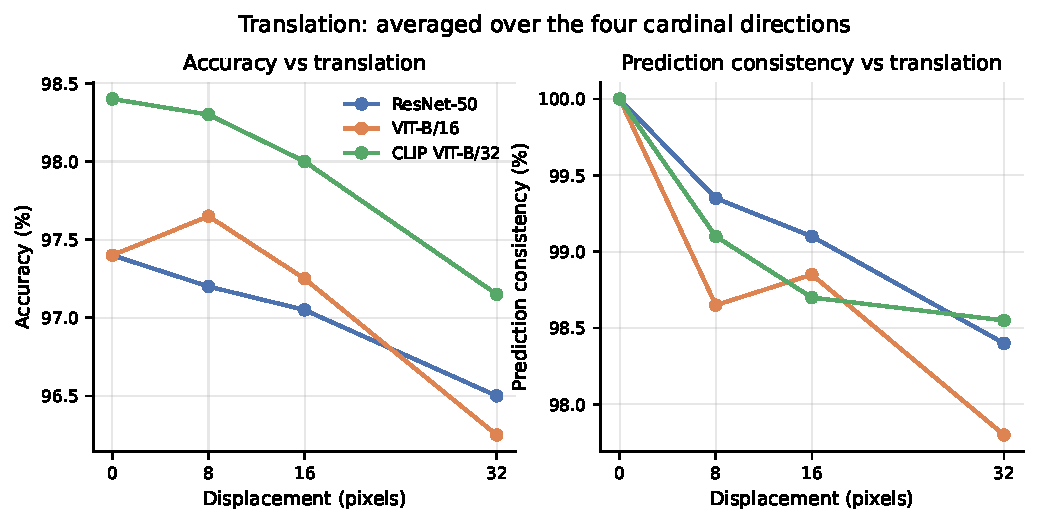
\includegraphics[width=\textwidth]{task1/translation_curve.pdf}
  \caption{Accuracy and prediction consistency against translation
  displacement, averaged over the four cardinal directions.}
  \label{fig:t1-translation}
\end{figure}

\subsection{RQ1}

A CNN uses kernels to scan the image in local patches, so texture, which is a
local statistic, is cheap to use as a cue, while shape exists only at object
scale and must be built up over many layers. ResNet-50 should therefore lean
on surface cues, and it does, with the largest colour gap at 2.6 percentage
points and the lowest shape bias at 56.21\%, barely better than a guess. A
ViT instead applies self-attention across patches, so every patch is
represented with reference to all others from the first layer onward, making
global structure available immediately, which its shape bias of 79.31\%
reflects. CLIP shares that architecture but is trained to match images
against captions, and a plausible caption reads ``a german shepherd catching
a ball'' rather than ``a german shepherd with a brown patch'', so object
identity and action are what its representation must encode, giving it the
highest shape bias at 82.78\% and the smallest colour gap at 0.2 percentage
points. The fact that two independent interventions produce the same ordering
is stronger evidence than either in isolation. Coverage is close across the
three at 64.02\%, 60.67\% and 63.18\%, a spread of 3.35 points, so the
comparison is not distorted by one model deciding on far fewer images, but at
60\% to 64\% roughly a third of conflicts resolved to neither intended class,
and ResNet-50's 86 other decisions equal its 86 shape decisions, so its
56.21\% rests on a thin margin.

\subsection{RQ2}

Translation changes only absolute position but preserves relative
arrangement, which convolution handles by design. ResNet-50 degrades least at
$-0.028$ accuracy percentage points per pixel, against ViT-B/16's $-0.040$
and CLIP's $-0.041$, matching the prediction that the learned absolute
position embeddings of ViT offer no guarantee equal to convolution.
Translation causes a small accuracy drop in absolute terms, with all three
losing between 0.90 and 1.25 points across the full 32 pixel range. Patch
shuffling reverses the ordering. It preserves every pixel and destroys only
relative arrangement, so the kernels still work but deeper layers of
ResNet-50 detect relationships by reading spatial closeness of patches, which
shuffling makes false, and its accuracy drops by 8.8 against the 7.0 loss of
ViT-B/16, whose attention recomputes which patches relate by content at every
layer. CLIP loses 14.6 despite sharing ViT architecture, so architecture
alone does not account for robustness here. In terms of confidence, ResNet-50
retains 94.0\% of its clean confidence while losing 8.8 points in accuracy,
making it confidently wrong, whereas CLIP's falls to 72.7\%, so its misfires
are more clearly uncertain.

\subsection{RQ3}

Prediction accuracy asks how many images the model still gets right after an
intervention. Cosine stability asks how far the feature vector for each image
moved, by measuring the angle between its clean and transformed
representations. These can deviate, because a classifier does not need
feature vectors to stay in place, only to separate them. If every feature
vector shifts in the same direction, the boundary between classes still
holds, so stability is low and accuracy should not experience significant
change, and vice versa. Patch shuffling is where they disagree most.
ViT-B/16 has the lowest stability at 0.649 and the smallest accuracy drop at
7.0 points. CLIP has higher stability at 0.729 and the largest drop at 14.6
points. Thus, the two metrics do not show a tendency to agree. For zero-shot
against the linear head, CLIP encodes images and text into one shared space,
so a class can be represented either by a weight vector learned from labels
or by an encoded prompt such as ``a photo of a cat''. Both are compared to
the image feature by dot product, so the two readouts differ only in where
the class vectors come from. The linear head's training did not create the
class separability, it was already present in the frozen backbone's features.
The backbone cannot change during probe training, and ten encoded prompts
reach 98.0\% against the head's 98.4\% while agreeing on 99.0\% of individual
predictions, so the head is reading off structure rather than producing it.

\subsection{RQ4}

Only two comparisons here are controlled. ResNet-50 and ViT-B/16 share
pretraining data and supervision and differ mainly in architecture, so the
rise in shape bias from 56.21\% to 79.31\% can be attributed to the move from
local kernels to global attention. CLIP against the other two is not
controlled, since architecture, pretraining scale, supervision type and
augmentation all differ at once. Language supervision is the most plausible
account of its 82.78\% shape bias, but pretraining scale varies with it and
cannot be separated. Patch shuffling makes the limit clear, as CLIP loses
14.6 accuracy points against the 7.0 of ViT despite the shared architecture.

% ============================================================================
\section{Task 2: Unsupervised Domain Adaptation}
\label{sec:task2}

PACS provides Photo, Art and Cartoon as labelled sources and Sketch as an
unlabelled target. All four methods fine-tune the same ImageNet-pretrained
ResNet-18 and differ only in the loss term added to cross-entropy. DAN adds
an MMD penalty between source and target features. DANN adds a domain
discriminator with a gradient reversal layer, so the feature extractor is
trained to make the domains indistinguishable. CDAN uses the same
discriminator but feeds it the feature vector multiplied by the predicted
class probabilities. Checkpoints are selected on mean source-validation
macro-F1, and target labels are read only after every checkpoint is frozen.

\begin{table}[t]
  \centering
  \small
  \setlength{\tabcolsep}{4pt}
  \caption{PACS with Sketch as the target domain. Each source validation
  domain is reported before the mean, since pooling can hide source-specific
  behaviour. Separability is how well a probe can tell source features from
  target features, where 50.0 is chance. $\Delta$ is the change in target
  accuracy from Source-only. The lower block is the alignment-strength study,
  where $\lambda = 1$ is the same run as DAN.}
  \label{tab:t2-main}
  \begin{tabular}{lcccccccc}
    \toprule
    & \multicolumn{3}{c}{Source validation} & & & & & \\
    \cmidrule(lr){2-4}
    Method & Photo & Art & Cart. & Mean & Worst & Separ. & Target & $\Delta$ \\
    \midrule
    Source-only & 97.90 & 89.51 & 94.24 & 93.88 & 89.51 & 99.59 & 71.47 & --- \\
    DAN         & 96.70 & 92.93 & 94.46 & 94.69 & 92.93 & 83.52 & 58.56 & $-12.90$ \\
    DANN        & 95.20 & 92.93 & 93.60 & 93.91 & 92.93 & 98.63 & 80.55 & $+9.09$ \\
    CDAN        & 96.70 & 89.51 & 89.98 & 92.06 & 89.51 & 98.49 & 65.05 & $-6.41$ \\
    \midrule
    DAN $\lambda=0.1$  & --- & --- & --- & 95.10 & --- & 97.39 & 70.86 & $-0.61$ \\
    DAN $\lambda=1.0$  & --- & --- & --- & 94.69 & --- & 83.52 & 58.56 & $-12.90$ \\
    DAN $\lambda=10.0$ & --- & --- & --- & 21.68 & --- & 75.55 & 4.07  & $-67.40$ \\
    \bottomrule
  \end{tabular}
\end{table}

\begin{figure}[t]
  \centering
  \begin{subfigure}{0.49\textwidth}
    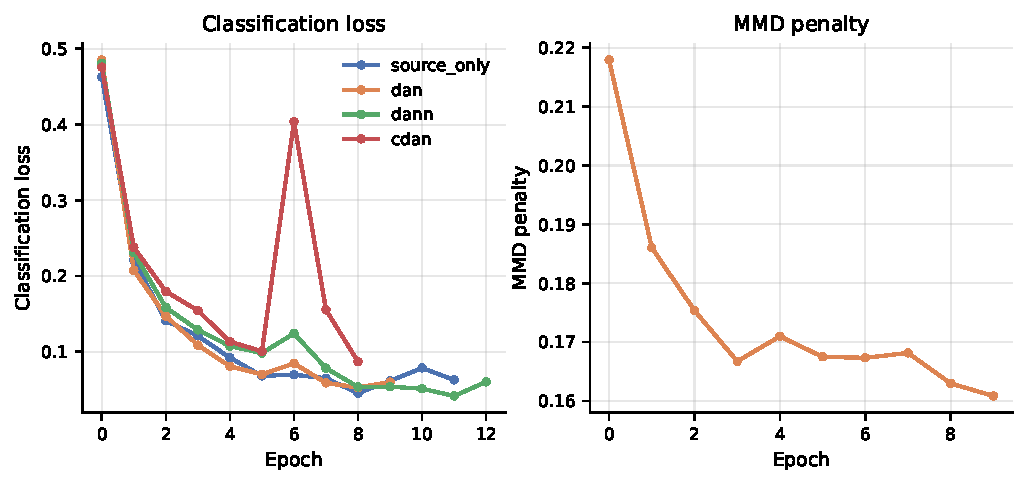
\includegraphics[width=\textwidth]{task2/training_curves.pdf}
    \caption{Four methods.}
  \end{subfigure}
  \hfill
  \begin{subfigure}{0.49\textwidth}
    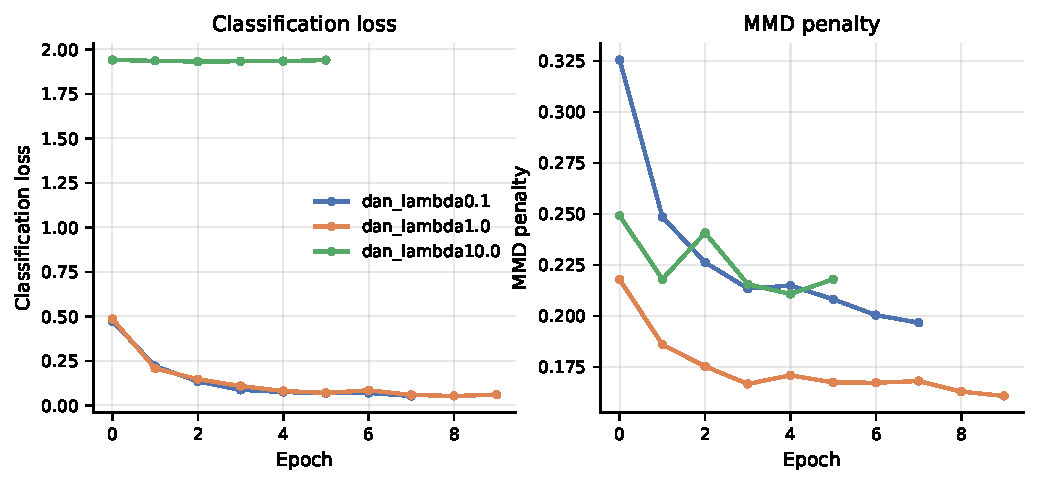
\includegraphics[width=\textwidth]{task2/lambda_study_curves.pdf}
    \caption{Alignment-strength study.}
  \end{subfigure}
  \caption{Classification loss and MMD penalty during training.}
  \label{fig:t2-curves}
\end{figure}

\subsection{RQ1}

Source-only ERM falls from 97.90\% accuracy on the Photo domain to 71.47\%
accuracy on the Sketch domain. The loss is not uniform across classes. The
largest confusions are dog predicted as horse 245 times, giraffe as horse 147
times, and dog as elephant 132 times, so horse acts as a sink class absorbing
errors from several sources. This fits a representation that loses the cues
separating four-legged animals once colour and texture are removed, leaving
outline as the only signal and defaulting to the most generic one. Reporting
the source domains separately shows further variation the mean conceals: the
Art domain reaches only 89.51\% accuracy against 97.90\% of Photo, so the
mean source accuracy of 93.88\% overstates performance on the weakest source.

\subsection{RQ2}

Lower domain separability did not produce better target recognition. The
relationship actually went the other way. DAN reduced separability furthest,
from 99.59\% to 83.52\%, and had the worst target accuracy at 58.56\%. DANN
had separability almost unchanged at 98.63\% and produced the only gain in
accuracy at 80.55\%. One mechanism consistent with this is that MMD is a
fixed statistic that can be reduced by degrading features rather than
aligning them, while an adversarial discriminator driven to chance (near
50\% accuracy) cannot be pushed further, so the pressure of DANN on the
representation is bounded.

\subsection{RQ3}

DAN and DANN match the marginal feature distribution, which cannot detect
whether the classes correspond. Two domains can overlap completely while
their class regions sit in each other's place. CDAN instead multiplies each
feature vector by its predicted class probabilities before the discriminator
sees it, which splits the representation into per-class blocks, so target
features must line up with source features of the same class rather than with
just the source cloud. Its per-class results are strongly split: house gains
26.25 accuracy points and person gains 23.13, while horse loses 33.95 and
elephant loses 15.68. This fits conditioning on predicted labels that are
themselves unreliable, since horse was already the sink class absorbing dog
and giraffe errors in the baseline. Where the prediction is right,
conditioning aligns genuine class correspondences and delivers gains in
accuracy the marginal methods do not. Where it is wrong, the objective pulls
target features toward the wrong class and reinforces the existing confusion.

\subsection{RQ4}

As $\lambda$ rises, source accuracy, separability and target accuracy all
fall together, so there is no one best setting. At $\lambda = 0.1$ the model
reaches 95.10\% source and 70.86\% target accuracy, just under the baseline's
71.47\%. At $\lambda = 1.0$ target falls to 58.56\%. At $\lambda = 10.0$ it
collapses to 21.68\% source and 4.07\% target, below the 14.3\% chance level.
The expected trade-off, paying source accuracy to gain target accuracy, never
appears, and the training curves show why $\lambda = 10.0$ fails completely:
classification loss stays flat at $\ln 7 \approx 1.95$, the score of a
uniform guess, while the MMD penalty ends higher than at $\lambda = 1.0$, so
the alignment term destroyed the classifier without minimising the penalty it
was weighted ten times to minimise. $\lambda$ weights the alignment term, and
MMD compares feature vectors, so training at any $\lambda$ needs target
images but not target labels. Choosing between the trained models is the part
that would need labels. Source accuracy ranks $\lambda = 0.1$, $1.0$ and
$10.0$ as 95.10\%, 94.69\% and 21.68\%, matching their target ordering of
70.86\%, 58.56\% and 4.07\%, so it would have chosen correctly.

% ============================================================================
\section{Task 3: Domain Generalization}
\label{sec:task3}

The protocol matches Task 2 exactly, except that no Sketch image is available
during training, diagnostics or checkpoint selection. ERM is Task 2's
Source-only checkpoint loaded unchanged rather than retrained, so both tasks
measure against identical baseline weights. DAN-DG applies the same MMD
penalty as DAN, but between every pair of source domains rather than between
source and target, since there is no target to align to. SAM wraps the same
optimiser in a two-pass update: it steps to the worst point within a radius
of 0.05, takes the gradient there, and applies it back at the original
weights.

\begin{table}[t]
  \centering
  \caption{PACS with Sketch never seen during training. Separability is a
  three-way probe over Photo, Art and Cartoon, where 33.33 is chance.
  $\Delta_{\text{sharp}}$ is how much validation loss rises after one small
  weight perturbation, so lower means the model sits in a flatter region.
  Chance accuracy for seven classes is 14.3.}
  \label{tab:t3-main}
  \begin{tabular}{lccccc}
    \toprule
    Method & Mean source & Worst source & Separability & $\Delta_{\text{sharp}}$ & Sketch \\
    \midrule
    ERM                  & 93.88 & 89.51 & 89.33 & 1.2796 & 71.47 \\
    DAN-DG ($\lambda=1$) & 21.68 & 17.27 & 54.67 & 0.3917 & 4.07 \\
    SAM                  & 95.88 & 94.63 & 85.33 & 0.1960 & 71.57 \\
    \midrule
    DAN-DG $\lambda=0.1$  & 95.50 & 93.90 & 70.33 & 0.3071 & 71.67 \\
    DAN-DG $\lambda=10.0$ & 21.68 & 17.27 & 58.33 & 0.2598 & 4.07 \\
    \bottomrule
  \end{tabular}
\end{table}

\begin{figure}[t]
  \centering
  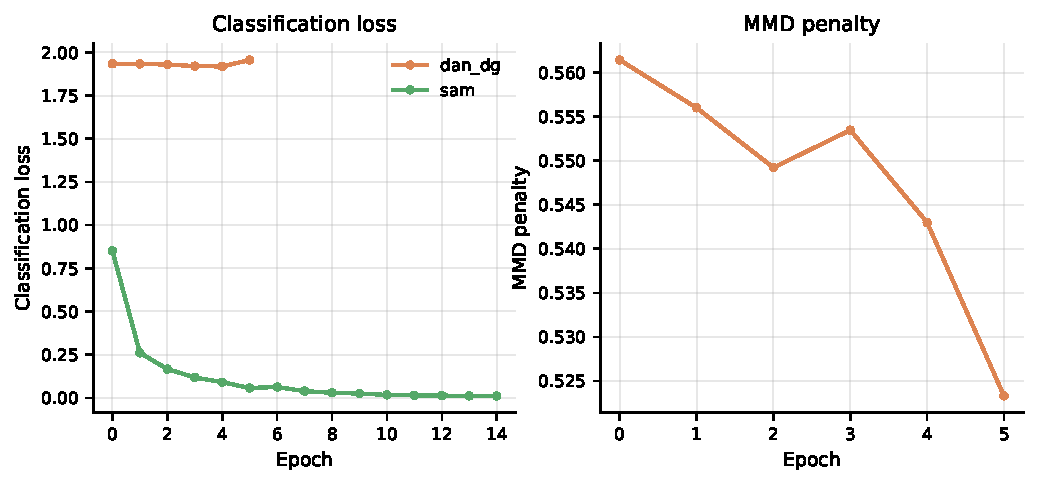
\includegraphics[width=0.85\textwidth]{task3/training_curves.pdf}
  \caption{Classification loss and MMD penalty for DAN-DG and SAM. DAN-DG's
  classification loss remains at $\ln 7 \approx 1.95$ throughout while its
  alignment penalty falls steadily.}
  \label{fig:t3-curves}
\end{figure}

\subsection{RQ1}

Source metrics tell you whether a model trained at all. They do not tell you
which working model will transfer better. DAN-DG at $\lambda = 1.0$ reaches
21.68\% mean source accuracy and 4.07\% on Sketch, so its failure is obvious
without ever looking at the target. SAM has the highest mean source accuracy
at 95.88\% and reaches 71.57\% on Sketch, against DAN-DG at $\lambda = 0.1$
with 95.50\% source and 71.67\% Sketch, differences one seed cannot resolve.
The aggregate also hides what happens per class. SAM's Sketch accuracy
differs from ERM's by 0.10 points, but it loses 25.63 points on person and
20.05 on giraffe while gaining 16.45 on guitar. Nothing in the source results
anticipates this, since SAM is the best model on every source domain.

\subsection{RQ2}

Making the source domains indistinguishable is easy if the model stops
encoding anything at all. That is what happened at the mandated setting.
Three-way source separability fell from 89.33\% to 54.67\%, close to the
33.33\% floor, so domain identity was nearly unreadable from the features.
Sketch accuracy fell to 4.07\%, below the 14.3\% floor for seven classes. The
training curves show it directly. Classification loss sits at
$\ln 7 \approx 1.95$ for every epoch, the score of a uniform guess, while the
MMD penalty falls steadily. The alignment objective was optimised and the
task was never learned. Mapping every feature to one point satisfies all
three pairwise MMD terms exactly, and the penalty cannot tell that apart from
genuine alignment. At $\lambda = 0.1$ separability falls to 70.33\% with
Sketch accuracy at 71.67\%, so the useful range ends before the mandated
setting.

\subsection{RQ3}

SAM reduced the sharpness proxy from 1.2796 of ERM to 0.1960, so it did what
it optimises. Whether that helps is a separate question, and here it did not.
DAN-DG measures flatter than ERM at 0.3917 while scoring 4.07\% on Sketch
against ERM's 71.47\%. SAM's much flatter minimum gives 71.57\%. The reason
DAN-DG looks flat is that a collapsed model has nothing left to disturb. If a
representation ignores its input, a small change in the weights cannot move
the loss much. A low proxy value is therefore not evidence of a good
solution. The proxy is also local by construction, as it measures the loss
increase after one climb step of magnitude 0.05 in one direction on one
batch.

\subsection{RQ4}

Both tasks share the same ERM baseline, so the comparison starts from
identical weights. Target-aware DAN reaches 58.56\% while target-free DAN-DG
reaches 4.07\% at the same $\lambda = 1.0$, which looks like a done case for
having target data. However, the two methods do not differ only in what they
see. DAN applies one MMD term between the pooled sources and the target.
DAN-DG applies three pairwise terms among the three source domains. At the
same $\lambda$ the alignment pressure in Task 3 is roughly three times
higher, so target access and alignment strength change together. DAN-DG at
$\lambda = 0.1$ reaches 71.67\%, above ERM, which supports that reading.

% ============================================================================
\section{Task 4: Open-Set Recognition}
\label{sec:task4}

CIFAR-10 is the known label set and sixteen fixed CIFAR-100 classes are held
out as unknowns, eight semantically near the known classes and eight far from
them. No unknown is seen during training, and every rejection threshold is
calibrated on CIFAR-10 validation data at 95\% known acceptance. Logits and
penultimate features are cached once per model, so all four scores read
identical outputs and any difference between them comes from the score rather
than the forward pass.

\begin{table}[t]
  \centering
  \small
  \caption{Post-hoc scores on the frozen vanilla model. AUROC is reported for
  near, far and all unknowns. Rejection is the share of unknowns caught at
  the threshold calibrated to 95\% known acceptance.}
  \label{tab:t4-posthoc}
  \begin{tabular}{lccccc}
    \toprule
    & \multicolumn{3}{c}{AUROC (\%)} & \multicolumn{2}{c}{Rejection (\%)} \\
    \cmidrule(lr){2-4} \cmidrule(lr){5-6}
    Score & Near & Far & All & Near & Far \\
    \midrule
    MSP         & 81.56 & 90.18 & 85.87 & 26.12 & 40.25 \\
    MLS         & 79.95 & 90.05 & 85.00 & 30.50 & 49.50 \\
    Energy      & 79.95 & 90.11 & 85.03 & 31.25 & 50.88 \\
    Mahalanobis & 79.80 & 92.21 & \textbf{86.01} & 26.00 & 51.88 \\
    \bottomrule
  \end{tabular}
\end{table}

\begin{table}[t]
  \centering
  \small
  \caption{Vanilla, GCSC and PROSER compared with MLS as the common score,
  plus PROSER's own placeholder-based score as an additional row. CSA is
  closed-set accuracy on CIFAR-10 test, computed from the ten known-class
  logits alone.}
  \label{tab:t4-models}
  \begin{tabular}{llcccccc}
    \toprule
    & & & \multicolumn{3}{c}{AUROC (\%)} & \multicolumn{2}{c}{Rejection (\%)} \\
    \cmidrule(lr){4-6} \cmidrule(lr){7-8}
    Model & Score & CSA & Near & Far & All & Near & Far \\
    \midrule
    Vanilla & MLS    & 94.83 & 79.95 & 90.05 & 85.00 & 30.50 & 49.50 \\
    GCSC    & MLS    & \textbf{95.02} & 82.02 & 91.89 & \textbf{86.95} & 35.62 & 60.50 \\
    PROSER  & MLS    & 94.58 & 78.80 & 88.21 & 83.51 & 29.25 & 46.00 \\
    PROSER  & PROSER & 94.58 & 76.47 & 91.87 & 84.17 & 25.50 & 57.50 \\
    \bottomrule
  \end{tabular}
\end{table}

\begin{figure}[t]
  \centering
  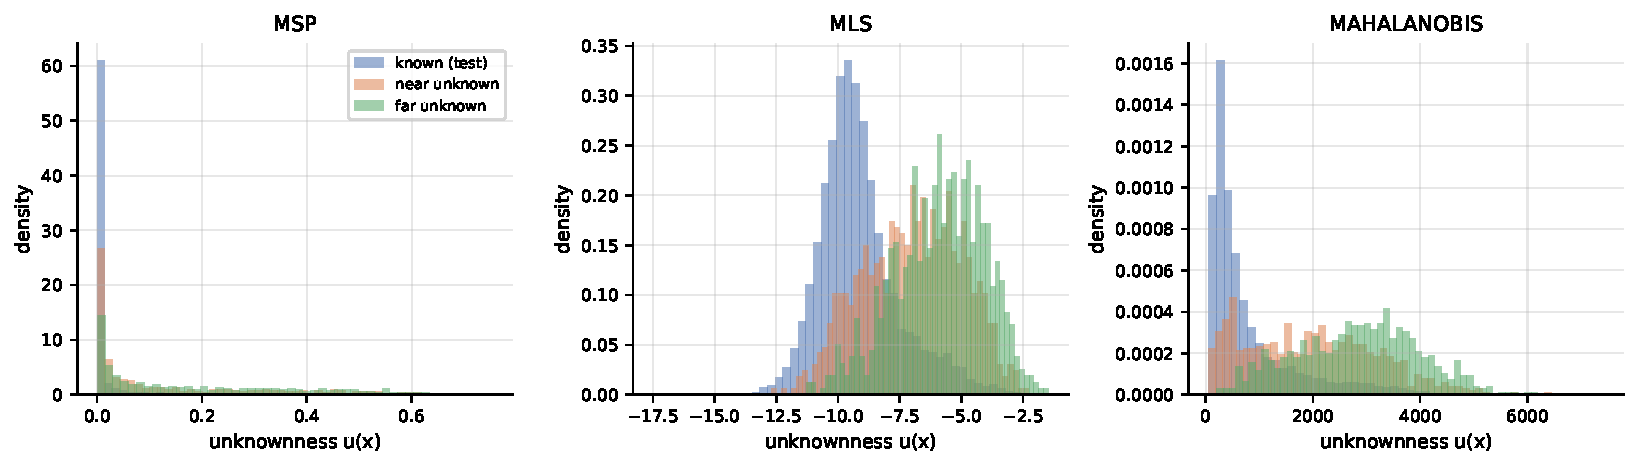
\includegraphics[width=0.9\textwidth]{task4/score_distributions.pdf}
  \caption{Score distributions for known and unknown inputs.}
  \label{fig:t4-scores}
\end{figure}

\subsection{RQ1}

How close an unknown is to the known classes controls whether it gets
classified as a known. Near-unknown AUROC is 80.31\% against 90.64\% for far
unknowns on the vanilla model, and that trend holds for all three models.
Near failures make sense: bus predicted as truck, pickup-truck as automobile,
fox as dog, all cases where the unknown shares its most prominent features
with the predicted class and CIFAR-10 has nothing better to offer. Far
failures do not: mushroom as cat, wardrobe as cat, bottle as cat, chair as
airplane, with cat absorbing three of the five far cases. These are not
borderline decisions either, since the bus case sits 6.97 points clear of the
rejection threshold on the accepted side.

\subsection{RQ2}

The four scores read different things. MSP measures confidence after softmax
and throws away logit magnitude. MLS keeps that magnitude. Energy adds up
evidence across all logits instead of taking the largest. Mahalanobis ignores
the logits and measures how far the feature vector sits from the nearest
class mean. The three logit scores agree closely, sitting within one point of
each other on the vanilla model and rising together under GCSC, so they are
three views of the same quantity rather than three signals. Mahalanobis is
the one that disagrees. It is best on the vanilla model at 86.01\%, and its
advantage is largest on far unknowns, where distance from every class mean is
exactly what an unrelated input produces. Under GCSC it falls to 84.82\% and
loses 2.25 points on near unknowns, moving from best to worst, because wider
class regions shorten the distance an unknown must travel to look familiar.
Feature distance is therefore most informative when classes are tightly
clustered and the unknown is distant, while the confidence-based scores hold
up better when training spreads the features out.

\subsection{RQ3}

GCSC improved closed-set accuracy from 94.83\% to 95.02\% and improved three
of the four rejection scores, with MSP, MLS and Energy each gaining about two
points of AUROC. Mahalanobis moved the other way and decreased 1.18 points.
One cause explains both. RandAugment forces many distorted views of a class
to share a label, which tightens the decision boundary the logit scores read,
and also widens each class region in feature space to hold those views. Wider
regions shorten the distance from an unknown to the nearest class mean, which
is what Mahalanobis measures. The near and far split follows from that.
Mahalanobis is reduced by 2.25 points on near unknowns and only 0.12 on far,
because widening the class regions costs the most where the unknown was
already close.

\subsection{RQ4}

No, for both cases. PROSER's placeholder loss reached 0.0000 by epoch 30, so
the objective was fully optimised, yet it scored below the vanilla baseline
it was fine-tuned from on every post-hoc score and about three points below
GCSC on the logit scores. It also decreased closed-set accuracy by 0.25, so
the CSA trade-off runs against it too. It does beat GCSC on Mahalanobis by
0.76 points, which fits placeholders tightening the boundaries between known
classes rather than widening them as augmentation does. Its own score locates
the failure, being weakest of the five on near unknowns at 76.47\% and
competitive on far at 91.87\%. The objective only ever asks a dummy to
outrank the runner-up once the true class is masked, so a dummy calibrated
above typical second-place logits satisfies it without detecting anything.
That clears the weak logits a far unknown produces but not the confident
response a near unknown produces. The mixup term was meant to cover this, but
a near unknown is not a point on the line between two known classes. This is
a reproduction at published defaults with one seed, so the claim is that
PROSER did not improve rejection here, not that the method does not work in
general.

% ============================================================================
\section{Cross-task Discussion}
\label{sec:cross}

\subsection{Visual cues and distribution shift}

Sketch removes exactly the cues Task 1 measures reliance on. It has no
colour, almost no texture, and preserves only outline. Task 1 found ResNet-50
the most colour-dependent and least shape-biased of the three backbones, so a
model with that profile should suffer most on a shift of this kind. The Task
2 confusions are consistent with it: once colour and texture are gone, dog is
predicted as horse 245 times and giraffe as horse 147 times, with horse
absorbing errors from several classes at once. This is a qualitative link
rather than a causal one. Task 1 uses STL-10 with frozen backbones while
Tasks 2 and 3 fine-tune a ResNet-18 on PACS, so the two settings share no
dataset, no architecture and no training procedure, and the pattern cannot be
tested directly without running Task 1's interventions on the PACS models.

\subsection{Invariance versus discriminability}

The two DAN-DG settings separate the useful case from the destructive one. At
$\lambda = 0.1$ separability falls from 89.33\% to 70.33\% while Sketch
accuracy stays at 71.67\%, slightly above ERM, so domain information was
removed without costing class information. At $\lambda = 1.0$ separability
falls to 54.67\%, close to the 33.33\% chance level, and Sketch accuracy
falls to 4.07\%, below the 14.3\% chance level, so the same objective pushed
further removed the class information as well. Task 2 shows the same pattern
with a different method, where DAN reduced separability furthest and had the
worst target accuracy of the four. The distinction is visible during training
without any target data. In the collapsed runs the classification loss sits
flat at $\ln 7 \approx 1.95$ from the first epoch while the alignment penalty
falls, so a classification loss that does not move while the penalty does is
the direct signal that alignment is being satisfied by discarding the task.

\subsection{The importance of target domain access}

Both tasks share the same ERM baseline, so the comparison starts from
identical weights. At $\lambda = 1.0$ target-aware DAN reaches 58.56\% on
Sketch while target-free DAN-DG reaches 4.07\%, which looks decisive. It is
not, because the two methods differ in what they align as well as in what
they see. DAN applies one MMD term between the pooled sources and the target.
DAN-DG applies three pairwise terms among the three source domains, so at the
same $\lambda$ the alignment pressure is roughly three times higher. Target
access and alignment strength vary together and cannot be separated here. The
sweep supports that reading, since DAN-DG at $\lambda = 0.1$ reaches 71.67\%,
above ERM and close to DAN at $\lambda = 0.1$ at 70.86\%. A clean test would
match the effective alignment strength rather than the nominal $\lambda$.

\subsection{Recognition versus rejection}

Improving closed-set accuracy does not reliably improve rejection. GCSC
raised closed-set accuracy from 94.83\% to 95.02\% and improved three of the
four rejection scores by about two points each, but Mahalanobis fell 1.18
points, so the answer depends on which score is used. PROSER is the clearer
case, since it optimised its placeholder objective to zero and scored below
the baseline it was fine-tuned from on every score while also costing 0.25
points of closed-set accuracy. The near and far split shows where abstaining
matters most. Near-unknown AUROC is about ten points below far-unknown AUROC
for every model, and at the calibrated threshold the vanilla model rejects
only 30.50\% of near unknowns against 49.50\% of far ones. A confident
prediction on an input that resembles a known class is exactly the case these
detectors handle worst, and it is also the case where a wrong answer is
hardest to notice.

% ============================================================================
\section{Conclusion}
\label{sec:conclusion}

The same pattern appears in three independent settings. DAN reduced domain
separability furthest and had the worst target accuracy of the four methods.
DAN-DG reduced source separability to near chance and produced below-chance
Sketch accuracy. PROSER drove its placeholder loss to zero and scored below
the baseline it started from. In each case the proxy objective was optimised
successfully and the goal it stood in for got worse, so progress on a proxy
is not evidence of progress on the task. SAM is a weaker fourth instance,
reducing the sharpness proxy by a factor of 6.5 for a Sketch difference of
0.10 points.

Taken together the four tasks suggest what a representation should keep and
what it should discard. It should preserve the structure that survives a
domain change, since shape bias and colour independence track the models that
transfer best, and it should discard surface statistics such as colour and
local texture, which Task 1 shows are the cues most easily removed by a shift
and which Sketch removes entirely. Invariance should be sought only up to the
point where class information survives, since both DAN-DG settings show the
same objective can remove domain information and class information by the
same mechanism, and the classification loss during training is the signal
that separates the two. An input should be rejected rather than forced into a
known class when no known class fits it well, but the Task 4 results show the
inputs most in need of rejection are the ones closest to the known classes,
and these are the ones every score handles worst.

The strongest positive result is that two independent interventions in Task 1
ranked the three backbones identically by their reliance on surface
appearance, which no single measurement would have established. Every
experiment was run once with a single seed, so differences of one or two
points should not be read as real, and the conclusions here rest on the large
effects rather than the small ones.

% ============================================================================
\bibliographystyle{plain}
\begin{thebibliography}{9}

\bibitem{geirhos2019}
R.~Geirhos, P.~Rubisch, C.~Michaelis, M.~Bethge, F.~A. Wichmann, and W.~Brendel.
\newblock ImageNet-trained CNNs are biased towards texture.
\newblock In \emph{ICLR}, 2019.

\bibitem{huang2017}
X.~Huang and S.~Belongie.
\newblock Arbitrary style transfer in real-time with adaptive instance normalization.
\newblock In \emph{ICCV}, 2017.

\bibitem{radford2021}
A.~Radford et~al.
\newblock Learning transferable visual models from natural language supervision.
\newblock In \emph{ICML}, 2021.

\bibitem{long2015}
M.~Long, Y.~Cao, J.~Wang, and M.~I. Jordan.
\newblock Learning transferable features with deep adaptation networks.
\newblock In \emph{ICML}, 2015.

\bibitem{ganin2016}
Y.~Ganin et~al.
\newblock Domain-adversarial training of neural networks.
\newblock \emph{JMLR}, 17(59):1--35, 2016.

\bibitem{long2018}
M.~Long, Z.~Cao, J.~Wang, and M.~I. Jordan.
\newblock Conditional adversarial domain adaptation.
\newblock In \emph{NeurIPS}, 2018.

\bibitem{foret2021}
P.~Foret, A.~Kleiner, H.~Mobahi, and B.~Neyshabur.
\newblock Sharpness-aware minimization for efficiently improving generalization.
\newblock In \emph{ICLR}, 2021.

\bibitem{zhou2021}
D.-W. Zhou, H.-J. Ye, and D.-C. Zhan.
\newblock Learning placeholders for open-set recognition.
\newblock In \emph{CVPR}, 2021.

\bibitem{hendrycks2017}
D.~Hendrycks and K.~Gimpel.
\newblock A baseline for detecting misclassified and out-of-distribution examples.
\newblock In \emph{ICLR}, 2017.

\bibitem{liu2020}
W.~Liu, X.~Wang, J.~Owens, and Y.~Li.
\newblock Energy-based out-of-distribution detection.
\newblock In \emph{NeurIPS}, 2020.

\bibitem{vaze2022}
S.~Vaze, K.~Han, A.~Vedaldi, and A.~Zisserman.
\newblock Open-set recognition: a good closed-set classifier is all you need?
\newblock In \emph{ICLR}, 2022.

\bibitem{cubuk2020}
E.~D. Cubuk, B.~Zoph, J.~Shlens, and Q.~V. Le.
\newblock RandAugment: practical automated data augmentation.
\newblock In \emph{CVPR Workshops}, 2020.

\end{thebibliography}

\end{document}
